\documentclass[12pt, a4paper]{article}
\usepackage[utf8]{inputenc}
\usepackage[IL2]{fontenc}
\usepackage[czech]{babel}

\usepackage[colorlinks=true]{hyperref}
\usepackage{graphicx}


%Nastavi hloubku obsahu \setcounter{tocdepth}{3}

\begin{document}
	\begin{titlepage}
		\begin{center}
			
\includegraphics{img/ZCULogo.pdf}\\[1cm]
			\textsc{\LARGE Západočeská univerzita v~Plzni}\\[0.1cm]
			\textsc{\Large Fakulta aplikovaných věd}\\[0.1cm]
			\textsc{\large Katedra informatiky a~výpočetní techniky}
			\vfill
			\textsc{\LARGE Semestrální práce KIV/UPS}\\[0.2cm]
			\Large{Síťová hra Oběšenec\\za použití protokolu UDP}
			\vfill
			Jaroslav Klaus\\
			A13B0347P\\
			jklaus@students.zcu.cz\\[0.2cm]
			\today, Plzeň
		\end{center}
	\end{titlepage}

	\tableofcontents
	\newpage

	\section{Zadání}
	Vytvořte hru, kterou může hrát více hráčů. Řešení musí obsahovat program serveru, který bude obsluhovat více klientů i her současně. Klient bude po opětovném přihlášení pokračovat tam, kde přestal. Program musí být odolný proti chybným zadáním a musí adekvátně reagovat na výpadky serveru i klientů. Klient bude naprogramován v jazyce \emph{Java} a server v jazyce \emph{C} nebo \emph{C++}. Konkrétně vytvořte hru \emph{Oběšenec} za použití protokolu \emph{UDP}.
	
	Program bude doplněn o zpracování statistických údajů (Počet odeslaných a přijatých zpráv a bytů, počet chybných zpráv, počet znovu odeslaných zpráv apod.). Dále nesmí chyby v komunikaci znemožnit případně znesnadnit používání grafického rozhraní klienta.
	
	\section{Popis hry}
	Hra Oběšenec je relativně populární a jednoduchá. Cílem hráčů je uhodnout slovo na základě znalosti jeho délky. Hráč, který je na řadě, hádá písmenko, které si myslí, že je obsaženo ve slově. Pokud má pravdu, hádá znovu, pokud ne, hádá další hráč v pořadí. Za každé špatně hádané písmeno se hráči přikreslí část obrázku šibenice s oběšencem (odtud název hry) a pokud se obrázek kompletní, znamená to prohru. Výhra znamená, že hráč uhodl poslední skryté písmenko a slovo je tak kompletní. Další možností je pokusit se uhádnout celé slovo. Pokud jej uhádneme, vyhráváme, pokud ne, prohráváme.
	
	\section{Protokol}
	Z důvodu použití protokolu UDP bude potřeba řešit možnost ztráty, případně duplicity zpráv, nebo jejich špatné pořadí a poškození dat během přenosu. To bude vyřešeno tak, že každý zpráva bude obsahovat pořadové číslo a bude se na něj vyžadovat odpověď. Možnost ztráty spojení bude vyřešena tak, že se zprávy budou posílat opakovaně, dokud nebudou potvrzeny, a pokud klient některou nepotvrdí do stanovené doby, bude prohlášen za odpojeného. Stejně tak pokud neodpoví server, bude prohlášen za nedostupný. Zároveň se bude jednou za čas posílat zpráva typu \emph{“ping”} proto, aby se zamezilo výpadku spojení během tahu, tedy v době, kdy se žádné zprávy nezasílají. Možnost poškození dat během přenosu bude vyřešena pomocí \emph{checksumy}.

	Komunikační protokol bude textový s oddělovačem \emph{‘;’}. Bude se skládat z pěti částí - čísla zprávy, typu zprávy, kontrolního součtu, velikosti dat a dat. Data budou jako oddělovač používat \emph{‘,’}. Klient bude pro jeho identifikaci serverem posílat v každé zprávě své jméno.
	
	\subsection{Typy zpráv a dat}
	Typ zprávy bude uveden číslem, u kterého bude dále popsán význam a naznačeno, jak budou vypadat data. Jako první v popisu bude uvedeno, zda bude paket od klienta na server (C), nebo od severu ke klientovi (S).
		\begin{enumerate}
		\item S, C, potvrzení doručení paketu\\
		S: číslo potvrzovaného paketu (int)\\
		C: jméno (string), číslo potvrzovaného paketu (int)
		\item S, ukončení hry z důvodu nedostupnosti hráče\\
		Data: jméno (string)
		\item C, žádost o připojení\\
		Data: jméno (string), počet soupeřů (int)
		\item S, odpověď na žádost o připojení\\
		Data:	0 pokud vše proběhlo v pořádku, 1 pokud je jméno ve hře a hraje, 2 pokud je jméno ve hře a je odpojené
		\item C, žádost o navázání přerušené hry\\
		Data: jméno (string)
		\item S, odpověď na žádost o navázání přerušené hry\\
		Data: stav hry = stav hry (int, pokud -1, tak znamená, že hráč nebyl v žádné hře nalezen), počet hráčů (int), stav hádaného slova (string), již hádaná písmena (string), počet špatně hádaných písmen (int)
		\item S, začátek hry\\
		Data: počet hádaných písmen (int)
		\item C, odpojuji se\\
		Data: jméno (string)
		\item S, oznámení o někom, kdo se odpojil\\
		Data: jméno (string)
		\item S, prohrál jsi\\
		Data: -
		\item S, oznámení o někom, kdo prohrál\\
		Data: jméno (string)
		\item S, vyhrál jsi (= konec hry, uhodl slovo)\\
		Data: -
		\item S, oznámení o někom, kdo vyhrál\\
		Data: jméno (string)
		\item S, jsi na tahu\\
		Data: -
		\item S, oznámení, kdo je na tahu (pro ostatní hráče)\\
		Data: jméno (string)
		\item C, tah\\
		Data: jméno (string), hádané písmeno (char)
		\item S, odpověď na tah\\
		Data: pozice s uhodnutými písmeny (string 0 a 1, kde 1 znamená shodu)
		\item S, oznámení tahu\\
		Data: jméno (string), písmeno (char), pozice s uhodnutými písmeny (string 0 a 1, kde 1 znamená shodu)
		\item C, hádám celé slovo\\
		Data: jméno (string), slovo (string)
		\item S, oznámení hádání slova\\
		Data: jméno (string), slovo (string)
		\item S, C, ping\\
		S: -\\
		C: jméno (string)
		\item S, oznámení o klientovi, který chvilku neodpovídá\\
		Data: jméno (string)
		\end{enumerate}
		
	\section{Implementace}
	Zde je popsána dekompozice, rozvrstvení, metoda paralelizace a další implementační záležitosti programů.
	
		\subsection{Server}
		Program serveru je rozdělen do několika částí a postup zpracování zpráv je založený na vzoru producent -- konzument. První část je soubor \emph{main.c}, ve kterém probíhá kontrola počtu zadaných parametrů a volají se funkce pro vytvoření socketu, bind socketu a spuštění hlavní části serveru, které jsou implementované v souboru \emph{server.c}. Při vytvoření socketu se kontroluje, zda je zadaná adresa platná a port v rozmezí 1 až 65535.
		
		V hlavní části server inicializuje některé potřebné proměnné a struktury a spustí vlákna konzumenta (ta, která zpracovávají příchozí zprávy) a jedno vlákno, které periodicky posílá zprávy typu \emph{“ping”} všem klientům. Poté přejde do nekonečné smyčky, ve které se vždy zablokuje při čekání za příchozí zprávu. Pokud zpráva dorazí, server se ji pokusí rozparsovat do struktury \emph{struct message} -- zjistí pořadové číslo, typ zprávy, checksum, velikost dat, data a jméno hráče, který zprávu poslal. Pokud se mu to podaří, přidá zprávu do seznamu \emph{struct list} a upozorní konzumenty na novou zprávu. Pokud ne, tak byla zpráva při přenosu poškozená, případně nastal timeout. Ještě je zkontrolován seznam odeslaných zpráv, ve kterém čekají zprávy na potvrzení. Pokud se nalezne zpráva, která nebyla potvrzena po určitou dobu, odešle se znovu a pokud nebude ani po několika pokusech potvrzena, klient bude prohlášen za nedostupného a hra bude ukončena.
		
		Další část programu obsahuje soubor \emph{communication.c}, který implementuje funkce podstatné jak pro komunikaci (např. odeslání zprávy, výpočet checksumy apod.), tak pro zpracování příchozích zpráv (např. kontrolu checksumy, kontrolu pořadového čísla, reakce na zprávy apod.). Vlákno konzumenta čeká blokované na semaforu, dokud není v seznamu příchozích nějaká zpráva. Tu ze seznamu vyjme a zpracuje. Nejprve zkontroluje checksumu, poté pořadové číslo zprávy, pokud vše souhlasí, odešle potvrzení a na zprávu zareaguje dle protokolu výše.
		
		Soubor \emph{game.c} obsahuje funkce pro práci se strukturami \emph{struct player} a \emph{struct game}, které uchovávají informace o hráčích a hrách. Mezi tyto funkce patří např. vytvoření nového hráče, přiřazení hráče do hry, vytvoření nové hry, zrušení hry, kontrola tahu hráče atd.
		
		Soubor \emph{list.c} obsahuje funkce pro práci se seznamy zpráv, jako přidání zprávy do seznamu, vyjmutí zprávy ze seznamu, nalezení a vyjmutí zprávy po zpracování potvrzení. Posledním souborem je \emph{structures.h}, který obsahuje definice používaných datových struktur.
		
		\subsection{Klient}
		Postup práce klienta je téměř identický jako ten na serveru. Liší se např. v tom, že zde existuje pouze jedno vlákno pro zpracování zpráv. Další vlákno slouží pro příjem zpráv, jiné pro odesílání \emph{"pingu"} a poslední k ovládání GUI.
		
		První částí je soubor \emph{Main.java}, který zkontroluje počet argumentů a vytvoří okno klienta. To je implementováno v souboru \emph{Window.java} a po jeho vytvoření se spustí výše zmíněná vlákna. Stav hry se zobrazuje pomocí textových upozornění v okně hry, které také obsahuje tzv. plátno (definované v \emph{Canvas.java}), ve kterém se vykresluje příslušná šibenice s oběšencem.
		
		Soubor \emph{Connection.java} uchovává informace o spojení a obsahuje metody pro komunikaci, jako např. odeslání a příjem zprávy.
		
		\emph{Receiver.java} představuje vlákno pro příjem zpráv. Jeho práce je téměř identická s tou, kterou provádí hlavní vlákno serveru -- čeká na příchozí zprávu, kterou přidá do seznamu, zkontroluje a případně znovu odešle nepotvrzené zprávy a v případě dlouho nepotvrzené zprávy oznámí nedostupnost serveru.
		
		Soubor \emph{ProcessMessage} reprezentuje vlákno konzumenta, které čeká nad semaforem a po přijetí zprávy ji zpracuje a reaguje na ni dle protokolu (viz výše). Průběh zpracování zprávy je opět téměř symetrický se serverovou stranou.
		
		Dále jsou zde dva soubory \emph{Message.java} a \emph{Game.java}, které slouží jako datové struktury.
		
	\section{Uživatelská příručka}
	Server je napsán v jazyce \emph{C} v operačním systému Linux a je k němu vytvořen příslušný \emph{Makefile}, kterým je možné server pomocí nástroje \emph{make} jednoduše přeložit. K přeložení je potřebná knihovna \emph{pthread} pro možnost vytvoření a práce s vlákny apod. Server se spouští se dvěma parametry, adresou pro naslouchání a portem, např.\\
	\texttt{./server INADDR\_ANY 10000}\\
	Ukončení serveru je možné provést zasláním signálu \emph{SIGINT} (stisknutí Ctrl + C).
	
	Klient je napsán v jazyce \emph{Java} za použití \emph{JDK 6} a fungovat by tedy měl jak v OS Linux, tak Microsoft Windows. Pro jeho přeložení je tedy potřeba \emph{JDK 6} nebo vyšší, pro spuštění by měl stačit \emph{JRE 6} nebo vyšší. Přiložen je soubor \emph{build.xml} pro automatický překlad nástrojem \emph{ant}, který se provede např. příkazem\\
	\texttt{ant jar}\\
	Vytvoří se soubor \emph{Hangman.jar}, který lze spustit např. příkazem\\
	\texttt{java -jar Hangman.jar localhost 10000}\\
	Z příkazu je vidět, že se klient spouští se dvěma parametry a to adresou serveru a portem serveru.
	
	Po spuštění vypadá klient jako na obrázku \ref{Klient}. Novou hru vytvoříme z nabídky menu \emph{Game}, \emph{New Game} a do dialogu \ref{NewGame} zadáme svou přezdívku a počet protihráčů. Server nás automaticky přiřadí do hry se stejným počtem protihráčů, případně takovou hru vytvoří. Hra se poté ovládá tak, že pokud jste na tahu, tak hádání provedete tak, že daný znak stisknete na klávesnici. Pokud chcete hádat celé slovo, stiskněte klávesu \emph{Enter}. Pokud se ze hry odpojíte, máte v blízké době šanci se do ní opět vrátit a to pomocí nabídky menu \emph{Game}, \emph{Reconnect}, kam zadáte svou původní přezdívku a budete vráceni do hry.
	\begin{figure}[ht!]
		\centering
		\caption{Klient}
		\label{Klient}
		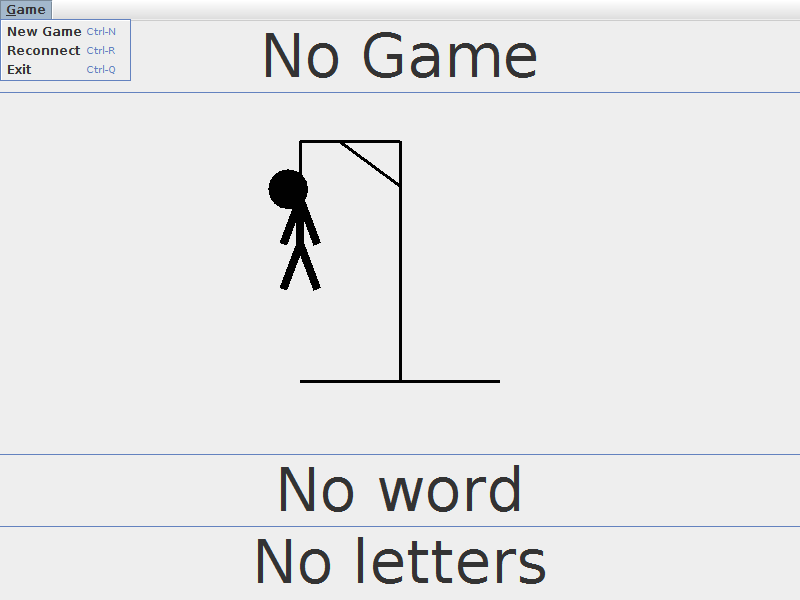
\includegraphics[width=13cm]{img/Client.png}
	\end{figure}
	\begin{figure}[ht!]
		\centering
		\caption{Nová hra}
		\label{NewGame}
		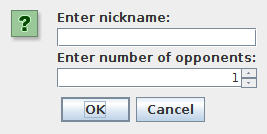
\includegraphics[width=6cm]{img/NewGame.png}
	\end{figure}
	\begin{figure}[ht!]
		\centering
		\caption{Reconnect}
		\label{Reconnect}
		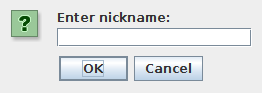
\includegraphics[width=6cm]{img/Reconnect.png}
	\end{figure}
	
	\section{Závěr}
	Vytvoření hry bylo mnohonásobně těžší, než jsem očekával. Zabralo mi relativně velkou spoustu času, cca 80 až 120 hodin. Jedním z důvodů bylo to, že nebylo jednoduché správně implementovat komunikaci pomocí UDP protokolu a také to, že jsem si při návrhu nedokázal uvědomit všechny možné problémy a situace, které mohou nastat. Přes to všechno si myslím, že jsem zadání splnil.
	
\end{document}